\chapter{Моделирование TGE и TGF
}\label{ch:thunderstorm}

\section{Обзор экспериментальных результатов
}\label{sec:thunderstorm/review-exp}


% Статья Chubenko2000.pdf - наблюдение рентгеновского излучения на Тяньшане
% Статья Chubenko2003.pdf - рост числа электронов в спокойной фазе без вспелесков гамма-квантов на Тяньшане
% Статья Chubenko2009.pdf - измерение спектра TGF на Земле
% Статья Antonova2007.pdf - появление радиосигналов при прохождении ШАЛ через грозу, в отсутвии ШАЛ радиосигнала нет.
% Статья Antonova2009.pdf - появление радиосигналов и гамма эмиссии скорелированной с прохождением ШАЛ через грозу и разрядами, в отсутвии ШАЛ радиосигнала нет.
% Gurevich2000.pdf --- даны оценки числа рожденных электрон-позитронных пар
% Gurevich_etal2013.pdf - Приведены результаты одновременных измерений радио и гамма-излучения во время гроз. Гамма-детектор, расположенный на высоте 3840 м, и два радиодетектора Тянь-Шаньской горной научной станции (высота 3340 м) регистрировали интенсивные гамма-вспышки и радиоимпульсы в момент возникновения молнии. В начальный момент времени (несколько сотен микросекунд) радиогамма-корреляция резко нарастает, а коэффициент корреляции достигает 0,9–0,95. Спектр гамма-энергии, измеренный при возникновении молнии, близок к характерному спектру пробоя на убегающих электронах. Наблюдаемые при этом радиоимпульсы имеют наибольшую амплитуду. Совместное наблюдение гамма-излучения и радиоизлучения подтверждает концепцию возникновения молнии из-за множественных одновременных электрических разрядов на гидрометеорах, стимулированных и синхронизированных низкоэнергетическими электронами, генерируемыми в процессе разгона. 
% Gurevich2001.pdf -- рсчеты гуревича для неоднороного поля, добавить в раздел про реактор
% Gurevich2002.pdf ---расчеты Гуревича для радиоимпульса от ШАЛ в грозе
% Gurevich2003.pdf --- наблюдение радиосигнала соотвевующего расчетам из Gurevich2002.pdf 
% Gurevich2011_background.pdf --- наблюдения TGF на Тянь-Шане.

\section{Обзор существующих моделей}\label{sec:thunderstorm/review-mod}

\subsection{Пробой на убегающих электронах}\label{sec:thunderstorm/gurevich}
%
Пробой на убегающих электронах (ПУЭ) --- модель развития лавины релятивистских (с энергией 0.1 --- 10 МэВ) электронов в постоянном электрическом поле предложенная А.~В.~Гуревичем~\cite{gurevich1992runaway,Gurevich2001ufn}. Качественно идея модели проста: пусть электрон ускоряется за счет электрического поля и тормозится за счет взаимодействия со средой, если он получает от поля больше энергии чем теряет, то у него появляется избыток энергии, который может быть потрачен на рождение нового электрона. Такие электроны будем называть убегающими. Если пренебречь всеми процессами кроме ионизационных потерь и радиационных потерь, то график ~\ref{fig:storm:gurevich}а показывает условия генерации лавины убегающих электронов в однородном поле. Энергию при которой электрон в среднем на единице длинны приобретает энергии больше чем теряет мы будем называть критической (зависимость её от высоты\footnote{Если не указано иное, Для установления значения плотности воздуха на разных высотах в моделировании используется международная стандартная модель атмосферы (ISA)} приведена на рис. ~\ref{fig:storm:gurevich}б).

\begin{figure}[t]
    \begin{center}
        \begin{minipage}[h]{0.49\linewidth}
            \center{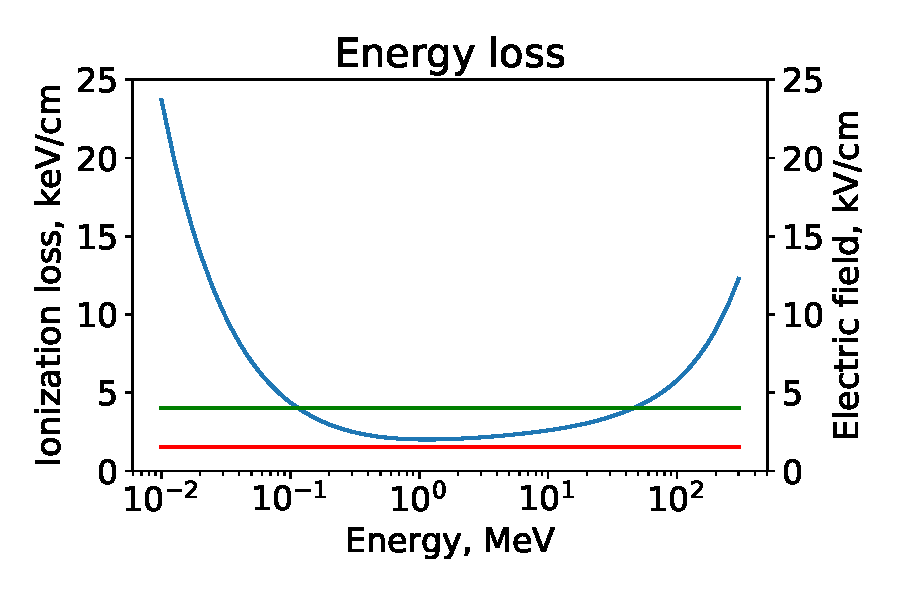
\includegraphics[width=\linewidth]{thunderstorm/01_Gurevich.pdf} \\ а)}
        \end{minipage}
        \hfill
        \begin{minipage}[h]{0.49\linewidth}
            \center{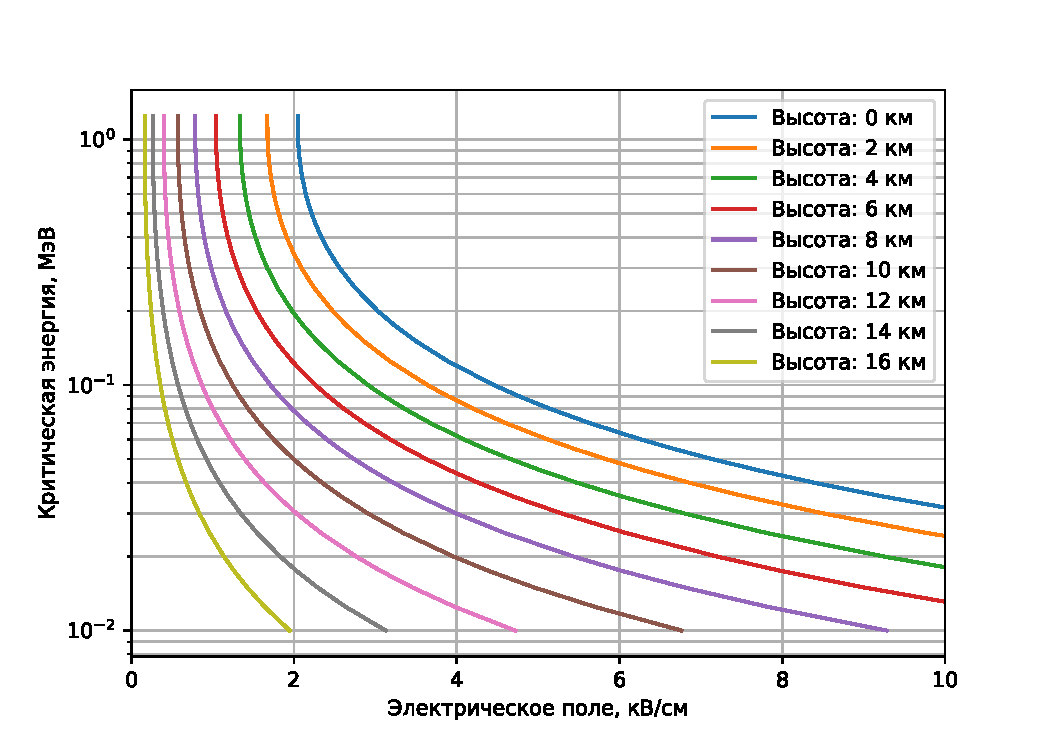
\includegraphics[width=\linewidth]{thunderstorm/02_CriticalEnergy.pdf}   \\ б)}
        \end{minipage}
        \caption{а) Ионизационные потери электронов в воздухе при нормальных условиях. б) Зависимость критической энергии от поля для различных высот.}
    \end{center}
    \label{fig:storm:gurevich}
\end{figure}

\section{Расчет числа убегающих электронов}\label{sec:thunderstorm/rrea}

Несмотря на то что есть достаточно консистентные оценки количества частиц в лавинах убегающих электронов~\cite{moss2006, DwyerSmith2005, skeltved2014, Gurevich2001ufn, Dwyer2012}, отдельные авторы~\cite{Oreshkin_2018} дают на порядки превосходящие оценки. Что бы уточнить этот вопрос, мы проведем собственные расчеты. Простая аналитическая оценка числа убегающих электронов может быть получена из элементарной теории ПУЭ~\cite{Gurevich2001ufn}. Давайте рассмотрим развитие электронной лавины в однородном электрическом поле. Согласно~\cite{Gurevich2001ufn} число убегающих электронов в RREA возрастает экспоненциально вдоль оси z:
\begin{equation}
\label{storm:exp}
N(z) = N_0 \cdot e^{\frac{z}{l_a}},
\end{equation}
где $l_a$ --- характерная длина нарастания электронной лавины, которая может быть оценена по следующей формуле:
\begin{equation}
l_a = a\frac{2 m c^{2}}{e} \frac{1}{E},
\end{equation}
где $m$ --- масса электрона, $c$ --- скорость света, константа $a \approx 11$, $E$ --- электрическое поле (для электронов с энергиями выше 80 МэВ, начинают доминировать радиационные потери, но тем не менее эта формула может дать оценку сверху). В качестве альтернативы мы можем использовать эмпирическую формулу полученную в стимуляциях Дваера~\cite{Dwyer2007}:
\begin{equation}
\label{storm:dwyer}
l_a = \frac{7300 kV}{E - 276 \frac{kV}{m} \cdot \frac{n}{n_0}},
\end{equation}
где $E$ --- электрическое поле, $n$ - концентрация воздуха, $n_0$ --- концентрация воздуха при н. у. Используя эти формулы, можно рассчитать число релятивистских электронов в зависимости от размера области с поле и величины поля. Результаты расчетов для высоты 10~км представлены на графике ~\ref{storm:number_runway}а, из него видно для максимально возможных условий на данной высоте (регион с полем не превышает 1200~метров, а электрическое поле~200 кВ/м) количество электронов не превышает $10^{10}$.

\begin{figure}[t]
    \begin{center}
        \begin{minipage}[h]{0.49\linewidth}
            \center{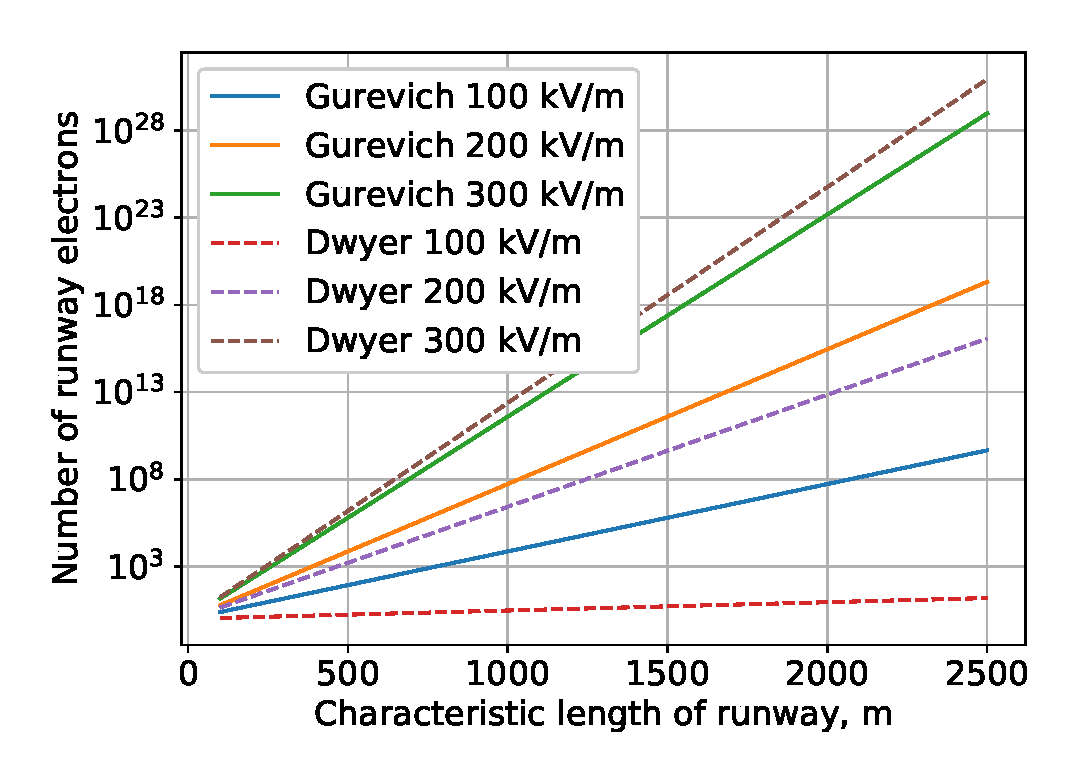
\includegraphics[width=\linewidth]{thunderstorm/epl2020/gurevich.eps} \\ а)}
        \end{minipage}
        \hfill
        \begin{minipage}[h]{0.49\linewidth}
            \center{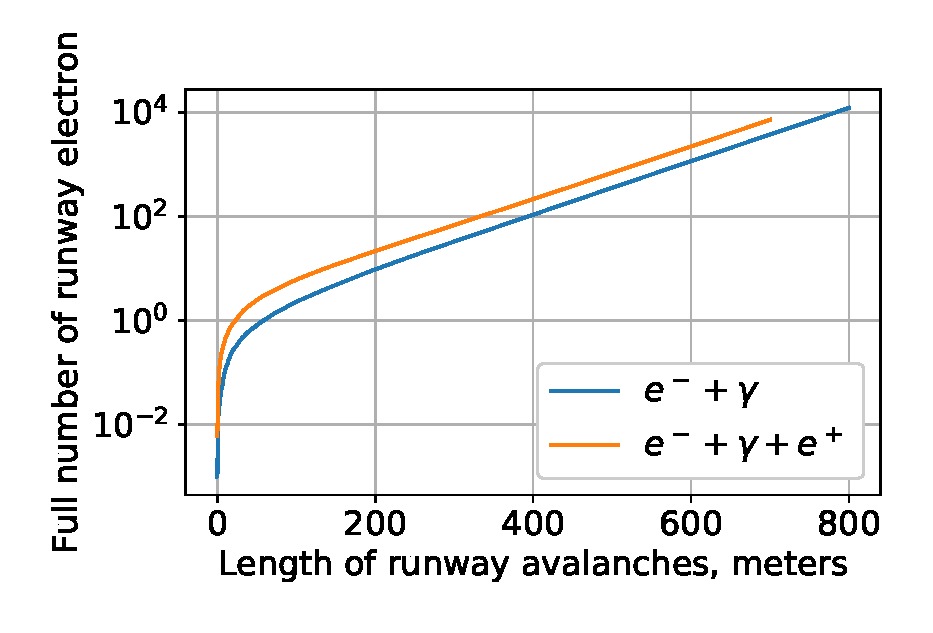
\includegraphics[width=\linewidth]{thunderstorm/epl2020/simulation.eps}   \\ б)}
        \end{minipage}
        \caption{  а) Число убегающих электронов в лавине в зависимости от длинны лавины. б) Число убегающих электронов из GEANT4 симуляции: синяя линия --- симуляция без позитронов, оранжевая --- с позитронами.}
    \end{center}
    \label{storm:number_runway}
\end{figure}
Более точные значения можно получить с помощью Монте-Карло моделирования лавины в электрическом поле с помощью GEANT4~\cite{Geant2003,Geant2006, Geant2016} (в данном разделе приведены расчеты с использованием версии 4.10.05).
Моделирование было проведено для следующих параметров: 
\begin{itemize}
    \item Область с полем представляет собой  цилиндр с шириной много большей его толщины, электрическое поле и плотность воздуха однородны;
    \item Плотность воздуха --- 0.4~кг/м~$^3$ (соответствует атмосферному давлению в  $\sim 0.25$~атм или высоте 10~км от уровня моря);
    \item Электрическое поле --- $200$~кВ/м (это максимальное электрическое поле обычно измеряемое в облаках~\cite{rakov_uman});
    \item Размер области с полем --- $800$~м для симуляции без позитронов и $700$~м для симуляции с позитронами (как мы увидим позже эти длины примерно соответствуют 10 характерным длинам нарастания лавины, что позволяет признать эти длины достаточными);
    \item Минимальный порог для рождения частиц --- 0.05 МэВ.
\end{itemize}
В каждой симуляции запускалось 1000 затравочных электронов (конечные результаты приведены на один электрон), результат симуляции приведен на рисунке~\ref{storm:number_runway}б. Результаты были фитированы функцией ~\ref{storm:exp}, в результате чего получены значения  $l_a \approx 85 m$ для симуляции без позитронов и $l_a \approx 78~m$ для симуляции с позитронами (для сравнения ~Eq.~\ref{storm:dwyer}~(формула Дваера) предсказывает $l_a \approx 64~m$). Используя полученную характерную длину можно оценить число убегающих электронов для разных длин, некоторые характерные значения приведены в таблице~\ref{tab:storm:approx}. На интересном нам участке $1200 - 1700$~метров рождает только $10^6-10^8$ убегающих электронов, что гораздо меньше числа $10^{16}$ предсказываемого в работе~\cite{Oreshkin_2018}, и сравнимо с оценками даваемыми другими авторами.
\begin{table}[h]
    \centering
    \begin{tabular}{crrr}
        \hline
        & & \multicolumn{2}{r}{Число убегающих электронов} \\
        &   Длина, м &   без позитронов &  с позитронами \\
        \hline
        \multirow{4}*{\rotatebox[origin=c]{90}{моделирование}} & 300 &  34.3      &  46 \\
        & 500 &  361     &  589 \\
        & 700 &  3802     &  7539 \\
        & 800 &  12350 &  --- \\
        \hline
        \multirow{5}*{\rotatebox[origin=c]{90}{экстраполяция}}& 1200 &  1.4e+06 &  4.3e+06 \\
        & 1700 &  5.0e+08 &  2.5e+09 \\
        & 2000 &  1.7e+10 &  1.2e+11 \\
        & 4000 &  2.9e+20 &  1.3e+22 \\
        & 5000 &  3.7e+25 &  4.5e+27 \\
        \hline
    \end{tabular}
    \caption{Оценка полного числа убегающих электронов основанная на симуляции в области размером 700-800 метров. Первая часть таблицы это взятые из симуляции, вторая часть это экстраполяция результатов моделирования.}
    \label{tab:storm:approx}
\end{table}

Результаты моделирования представлены в статье~\cite{zelenyi_2020}.












\clearpage